%%%%%%%%%%%%%%%%%%%%%%%%%%%%%%%%%%%%%%%%%%%%%%%%%%%%%%%%%%%%%%%%%%%%%%%%%%%%%%
%%%%%%%%%%%%%%%%%%%%%%%%%%%%%%%%%%%%%%%%%%%%%%%%%%%%%%%%%%%%%%%%%%%%%%%%%%%%%%
%%
%% Dokumentacia k projektu z IFJ
%% Autor: Martin Maga,Vit Mojzis, Viktor Malik, Vojtech Meca,Jiri Macku 
%% Datum: 27.11.2012
%%%%%%%%%%%%%%%%%%%%%%%%%%%%%%%%%%%%%%%%%%%%%%%%%%%%%%%%%%%%%%%%%%%%%%%%%%%%%%
%%%%%%%%%%%%%%%%%%%%%%%%%%%%%%%%%%%%%%%%%%%%%%%%%%%%%%%%%%%%%%%%%%%%%%%%%%%%%%
\documentclass[12pt,a4paper,titlepage,final]{article}
\newcommand{\uv}[1]{\quotedblbase #1\textquotedblleft}
% cestina a fonty
\usepackage[czech]{babel}
\usepackage[utf8]{inputenc}
% balicky pro odkazy
\usepackage[bookmarksopen,colorlinks,plainpages=false,urlcolor=blue,unicode]{hyperref}
\usepackage{url}
% obrazky
\usepackage[dvipdf]{graphicx}
\usepackage{listings} 
% velikost stranky
\usepackage{graphicx}
\usepackage[top=3.5cm, left=2.5cm, text={17cm, 24cm}, ignorefoot]{geometry}

\begin{document}

\begin{titlepage}

\begin{figure}[h]
\begin{center}
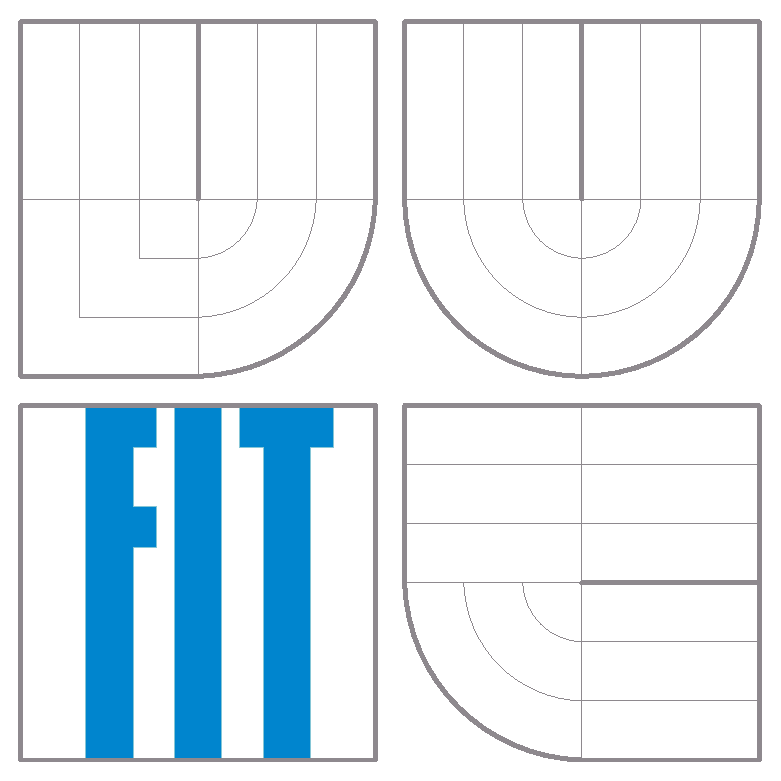
\includegraphics[scale=0.6]{logo.eps}
\end{center}
\end{figure}

\begin{center}
\LARGE
\textsc{Vysoké učení
  technické v~Brně\\ \Large{Fakulta informačních technológií}}\\
\vspace{\stretch{0.382}}
\LARGE
SHO Štátna volebná infraštruktúra \\
\Huge
Dokumentácia z predmetu IMS\\ 
\large{\medskip
\today }\\
\vspace{\stretch{0.618}}
\end{center}
 \hfill   

\begin{flushleft}
\begin{large}
\begin{tabular}{ll}
\textbf{Autori:} \\ \\

Martin Maga  xmagam00, \\Vojtěch Meca   xmecav00 \\ \\


\end{tabular}
\end{large}
\end{flushleft}
\end{titlepage}


\tableofcontents
\newpage

\section{Úvod}
Táto dokumentácia sa zaoberá vývojom, implementáciou a testovaním systéum hromadnej obsluhy "Štátna volebná infraštruktúra", ktorá simuluje volebný systém v Českej republike zahrňujúci voľby v okrskov a krajských mestskách a následne odoslanie a počítanie hlasov v informačnom centre.
\indent
Na základe modelu a simulácie bude ukázané chovanie systému so zreteľom na ukázanie slabých miest pri voľbách. Tento projekt môže byť použitý na optimalizáciu systému voliev v Českej republike vzhľadom na zrychlénie celého systému počítania hlasov a rozdelenie do okrskov.

\subsection{Autori}
Na projekte SHO "Štátna volebná infraštruktúra" sa podieľali nasledujúci autori:
\begin{itemize}
\item Martin Maga(xmagam00)
\item Vojtěch Meca(xmecav00)
\end{itemize}

Okrem vyššie spomenutých ľudí sme využili možňosť konzultácie s pánom doktorom Hrubým(konzultácia ohľadne správnosti nášho návrhu Petriho siete).

\subsection{Testovacie prostredie}
Pre testovacie účely boli použité architekrúry:Linux 3.2.0-56-generic $86_64$ GNU/Linux pre menšie vzorky dát a pre rozsiahlejšie testovanie na väčšej vzorke dát: FreeBSD eva.fit.vutbr.cz 9.2-STABLE FreeBSD amd64.

\subsection{Validita}
Experimentovaním sme overovali validitu modelu, ktoré vo forme histogramu a jeho následnej analýze odpovedali nášhu odhadovanému predpokladu. Tak isto sme využili dostupné informácie o spôsoboe volieb v Českej republiky a štatistických informáciách, ktoré sú verejne prístupné na internete.

\subsection{Zadanie}
Obsah zadania: "Státní volební infrastruktura nechť se skládá z volebního informačního centra a sítě volebních okrsků. Centrum přijímá zprávy od volebních okrsků a prezentuje výsledky v jednotlivých krajích (nutno modelovat server centra jako obslužnou linku). Volební okrsky jsou SHO obsahující obslužné linky: komise a místo pro provedení volby do obálky ("za plentou"). Modelujte proces příchodů voličů v průběhu doby voleb. Volební komise skončí práci buď po odvolení všech občanů v okrsku nebo okamžikem konce volebního víkendu. Potom sčítá hlasy (doba je závislá na počtu obálek v urně) a odesílá výsledky do centra. Prostudujte systém voleb v ČR a síť volebních okrsků. Konkrétní síť okrsků generujte náhodně s následujícím omezením: sumární počet voličů v krajích musí odpovídat realitě a počet voličů v krajských městech musí odpovídat realitě. Okrsky nějak vhodně agregujte tak, aby jejich celkový počet byl cca 200. Náhodně generovanou síť okrsků uložte do souboru a experimenty provádějte stále nad stejným modelem sítě okrsků. Zdokumentujte model sítě okrsků. Na experimentech ukažte propustnost centra, doby čekání okrsků na připojení do centra, celkovou dobu práce lidí okrskových komisích."
Obsah je dostupný online z nasledujúceho odkazu: http://perchta.fit.vutbr.cz:8000/vyuka-ims/31.\cite{Prokop:Algoritmy}



\subsection{Ciele projektu}
Ciele projektu zahŕňajú:
\begin{itemize}
\item Analýza aktuálneho volebného systému v Českej republike
\item Analýza slabých miest volebného systému
\item Návrh efektívnejšieho prístupu, ktoré by dokázalo zvýšiť rýchlosť počítania hlasov
\end{itemize}


\section{Rozber témy a použitých technológií}

\indent


Pre zobrazenie výsledkov bola použitá trieda Histogram, ktorá je štandardnou súčasťou knižnice Simlib.


\subsection{Popis použitých postupov}
Pre implementáciu bol zvolený jazyk C++ a knižnicu určenú na simuláciu Simlib. Toto rozhodnutie bolo učinené na základe formálnych požiadavok na tvorbu projektu. Ďalším kritériom bola aj široká ponuka prostriedkov, ktoré knižnica Simlib ponúka na simuláciu modelov. Ďalej treba spomenúť, že kód v C++ je pomerne rýchly.



\subsection{Pôvod použitých technológií}
\begin{itemize}
\item Simlib -http://www.fit.vutbr.cz/~peringer/SIMLIB/ (GNU LGPL)
\item C++ - http://en.wikipedia.org/wiki/C++
\item Ubuntu - http://www.ubuntu.com/
\item Petriho siete - $http://en.wikipedia.org/wiki/Petri_net$
\item GNU PLOT - $http://www.gnuplot.info/$

\end{itemize}
\subsection{Volebný systém v Českej republike}
Česká republika sa zaraďuje medzi dvojkomorové parlamentné 
systémy. Tvorí ju Poslanecká snemovňa a Senát. Do PS ČR sa volí na 
základe pomerného voličského systému. Základnú reguláciu nájdeme 
v Ústave ČR. V čl. 18 nachádzame základné princípy volieb, ako je spôsob 
voľby tajným hlasovaním na základe všeobecného, rovného a priameho 
práva, podľa zásad pomerného zastúpenia. Ďalším dôleţitým zákonom je 
zákon č. 247/1995 Sb., o voľbách. Niektoré ustanovenia sú prevedené 
vyhláškou č. 233/2000 Sb. Tieto právne pramene sú základnými právnymi 
prameňmi v oblasti volieb v ČR. 
 
Volebný systém za posledné roky pršiel určitými zmenami, jednou 
z nich bola zmena po voľbách v roku 1998. Zmena bola uzákonená v roku 
2000 na základe dohody ODS a ČSSD. Cieľom malo byť posilnenie 
stability a eliminácia vplyvu malých strán. Výsledkom tejto reformy bol 
pomerný systém, 35 volebných obvodov, v ktorých bola v jednom skrutíniu 
aplikovaná D 'Hontova formula.19
 Prezident Václav Havel šak nesúhlasil 
s polnením vetšinových prvkov vo volebnom systéme a navrhol Ústavnému 
súdu zrušenie zmien. Nálezom Ústavného súdu č. 64/2001 Sb. bola vetšina 
zmien zrušená. Ústavný súd argumentoval názorom, ţe došlo k vzájomnej 
kombinácii vetšinových prvkov a to narušuje ústavný príkaz pomerného 
zastúpenia v PS ČR. Vzhľadom k politickému rozloţeniu síl došlo k prijatiu 
nového zákona, ktorý si vyslúţil značnú kritiku od odbornej verejnosti. 
Štruktúra celého zákona prešla zmenou, zmenili sa velkosti obvodov, 
volebná formula, uzatváracia klauzula, počet aj charakter skrutínií. Pôvodná 
Hagenbach-Bischoffova volebná formula sa zmenila na D'Hotntovú. 
 
19
 Novák M., Lebeda T. a kol., Volební a stranické systémy. ČR v mezinárodním srovnání, 
Dobrá Voda: Vydavatelství a nakladatelství Aleš Čeněk, 2004, s. 231 
  34
D'Hontov deliteľ sa tak po vzore v celom svete s pomerným zastúpením 
dostal aj do českého zákona o voľbách. Uzatvárajúca klauzula ostala 
nezmenená, t.j. 5 \%, čo však neplatí pre koalície, kde sa priamo úmerne 
zvyšuje podľa počtu koaličných strán (zo 7 \% na 10 \%, z 9 \% na 10 \%, z 10 
\% na 20 \%). Počet skrutínií sa zmenšil z dvoch na jedno. D'Hontov deliteľ 
rozdeľuje všetky mandáty priamo na základe volebných obvodov, preto 
druhé skrutínium stratilo opdstatnenie.20
 Najvýznamnejšia bola ale zmena 
veľkosti volebných obvodov. Z pôvodných ôsmich vzniklo štrnásť , ktoré sú 
identické s krajským samosprávnym delením.21
 Kandidátske listiny ostali 
ako listiné, kde poradie kandidátov určuje politická strana. Volič má však 
právo na posun kandidáta na listine pomocou preferenčného hlasu, kde 
z pôvodných 4 došlo k zmene na 2 preferenčné hlasy. 
 
Zmenou volebného zákona došlo k posílneniu dvoch veľkých strán, 
avšak na druhej strane sa do parlamentu dostala aj relatívne malá Strana 
Zelených. Strany uprostred politického záujmu na základe tejto reformy 
oslabili. 

Odkaz:$http://is.muni.cz/th/108056/pravf-m-a2/Diplomova_prace.pdf$





\section{Koncepce - modelářska témata}

//treba dopisovat

\subsection{Opis konceptuálneho modelu}


\subsection{Forma konceptuálneho modelu}


\subsection{Implementácia}
Vzhľadom na koncepciu našeho interpretu sme sa rozhodli implementovať rozšírenie \emph{FUNEXP}. Vďaka nemu je interpret schopný spracovávať funkcie ako súčasť výrazov a tak isto výrazy použité, ako parametre funkcií. Jeho implementácia bola možná vďaka tomu, že parametre funkcií a tiež ich návratová hodnota sú predávané pomocou zásobníku interpretu. Preto je možné s týmito hodnotami pracovať pred a po volaní funkcie a počítať s nimi ako so súčasťou výrazov.




\section{Architektura simulačního modelu}
\newpage


\section{Podstata simulačných experimentov}

\section{Zhrnutie simulačných experimentov a záver}

\subsection{Testovanie}
Testovanie nášho projektu prebiehalo na architektúrach Windows a Linux. Bolo založené na vopred napísaných testoch, ktoré porovnávali jednotlivé výsledky testovanej časti s~referenčnými. Testovanie spočiatku prebiehalo po častiach, tak ako boli postupne implementované jednotlivé časti intepretu.
V~konečnej fáze boli vykonané komplexné testy, ktoré overili funkčnost nášho interpretu jazyka \emph{IFJ12} podľa špecifikácie uvedenej v~zadaní. V~prípade, že bola objavená chyba počas testovania, táto chyba bola ihneď odstránená a interpret bol opäť dôkladne otestovaný.


\subsection{Štatistiky}
\newpage


 
\newpage




\newpage

\section{Referencie}


\bibliographystyle{czechiso}

\bibliography{dokumentace}
\newpage
\end{document}

